\chapter{Bundle Adjustment}
\label{ch:bundle_adjustment}

\newenvironment{myindentpar}[1]
               {\begin{list}{}
                   {\setlength{\leftmargin}{#1}}
                 \item[]
               }
               {\end{list}}

\definecolor{lgray}{gray}{0.95}

Satellite position and orientation errors have a direct effect on the
accuracy of digital elevation models produced by the Stereo Pipeline.
If they're not corrected, these uncertainties will result in
systematic errors in the overall position and slope of the \ac{DEM}.
Severe distortions can occur as well, resulting in twisted or ``taco
shaped'' \acp{DEM}, though in most cases these effects are quite
subtle and hard to detect. In the worse case, such as with old mission
data like Voyager or Apollo, these gross camera misalignments can
prohibit Stereo Pipeline's internal interest point matcher and block
auto search range detection.

USGS's \ac{ISIS} software contains a suite of tools for correcting camera
position and orientation errors for their cameras using a process
called \emph{bundle adjustment}. Bundle adjustment is the process of
simultaneously adjusting the properties of many cameras and the 3D
locations of the objects they see in order to minimize the error
between the estimated, back-projected pixel location of the 3D objects
and their actual measured location in the captured images.

That complex process can be boiled down to this simple idea: bundle
adjustment ensures that observations in multiple different images of a
single ground feature are self-consistent. If they are not consistent,
then the position and orientation of the cameras as well as the 3D
position of the feature must be adjusted until they are.  This
optimization is carried out along with thousands (or more) of similar
constraints involving many different features observed in other
images.  Bundle adjustment is very powerful and versatile: it can
operate on just two overlapping images, or on thousands. It is also a
dangerous tool. Careful consideration is required to insure and
verify that the solution does represent reality.

\begin{figure}[bt]
  \centering
  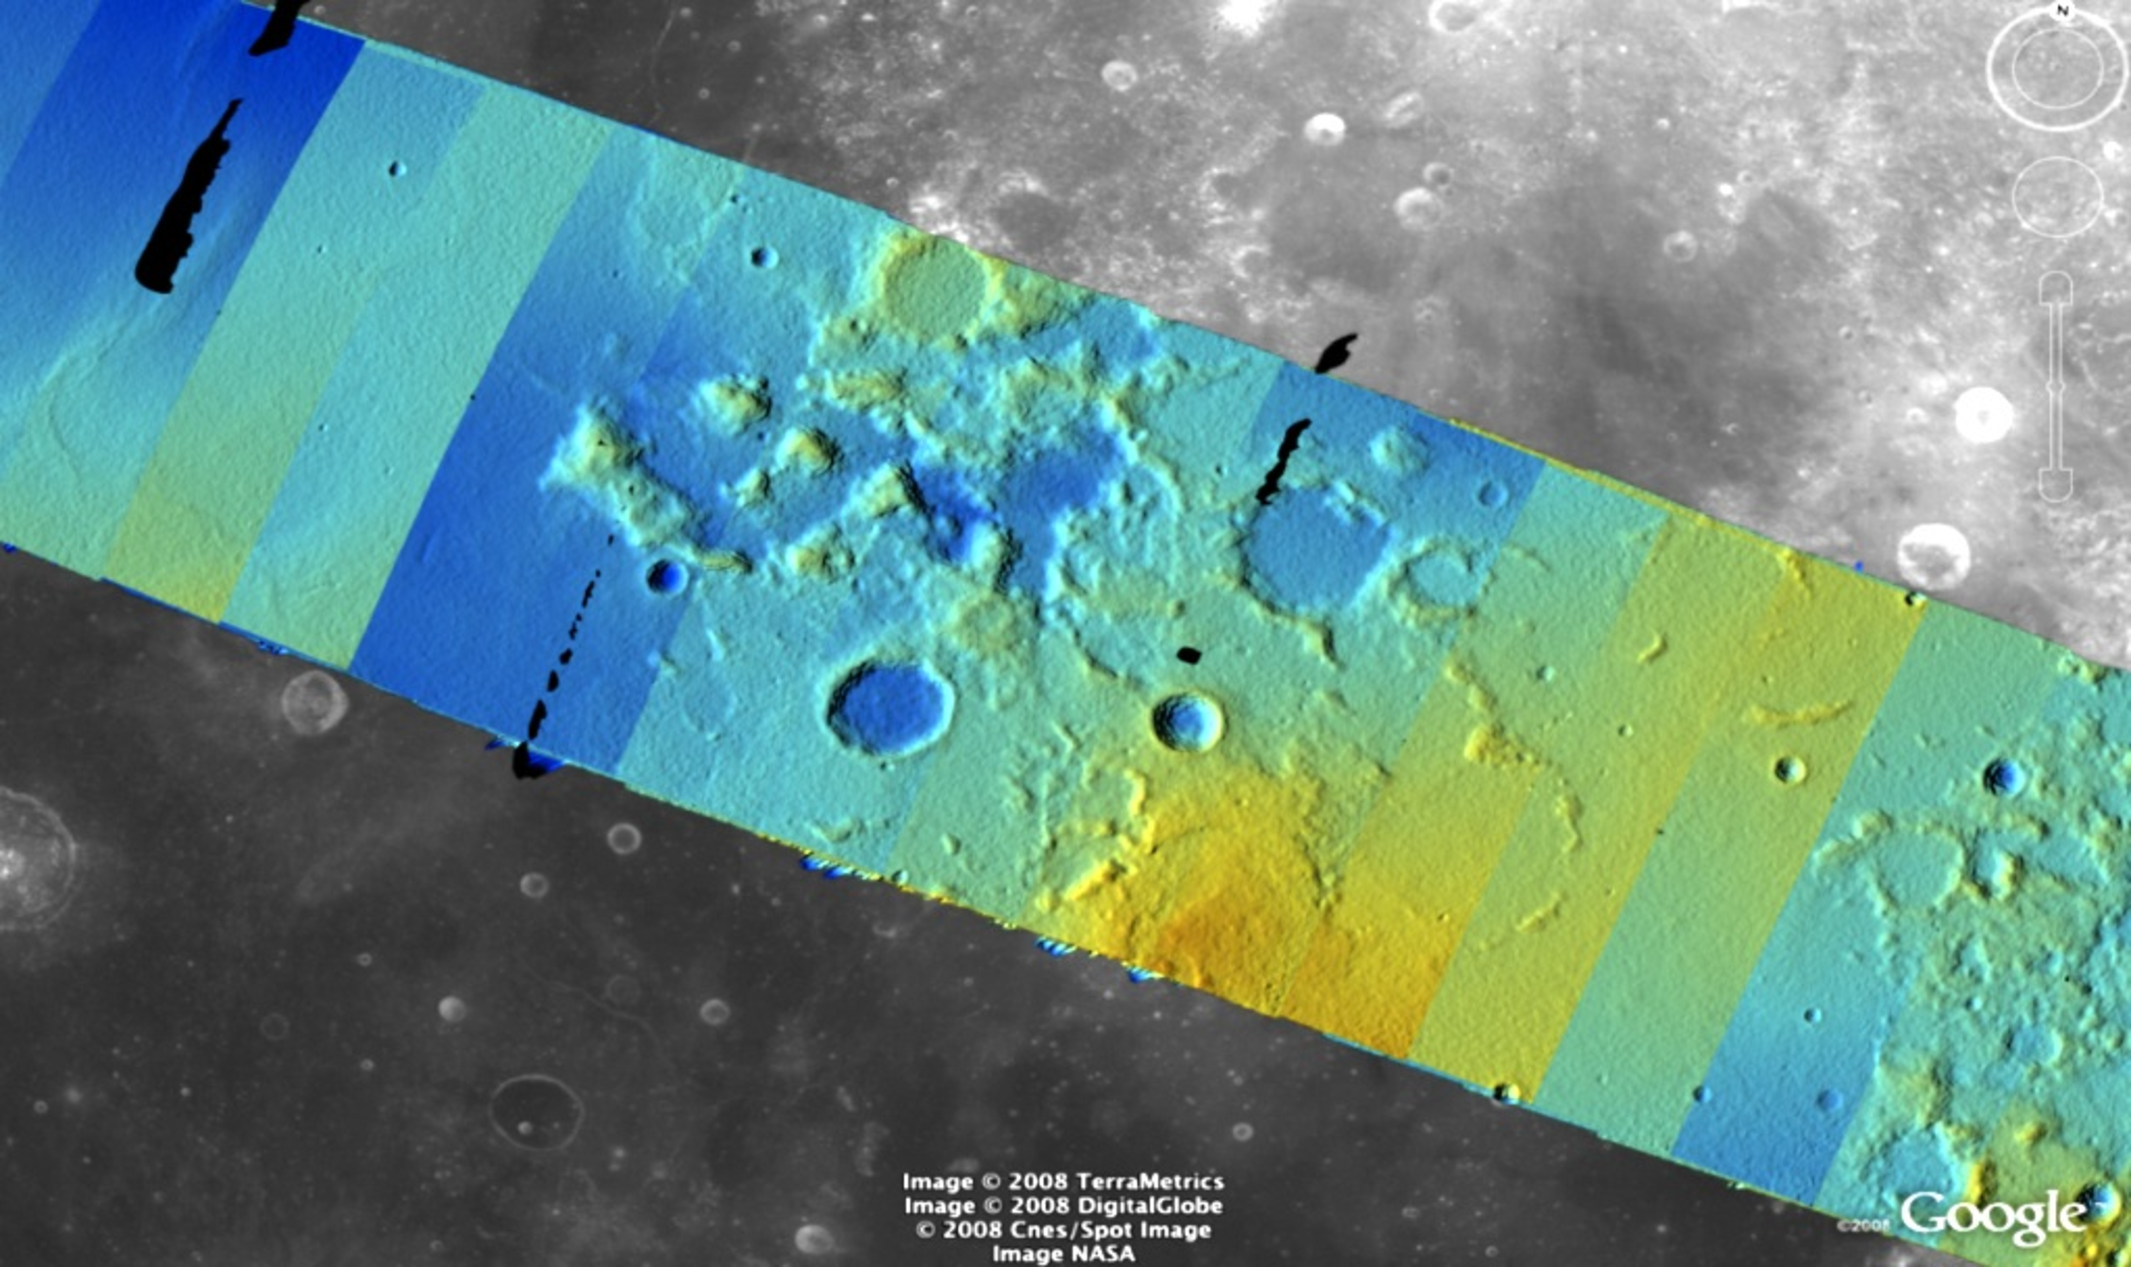
\includegraphics[width=8cm]{images/ba_orig}
  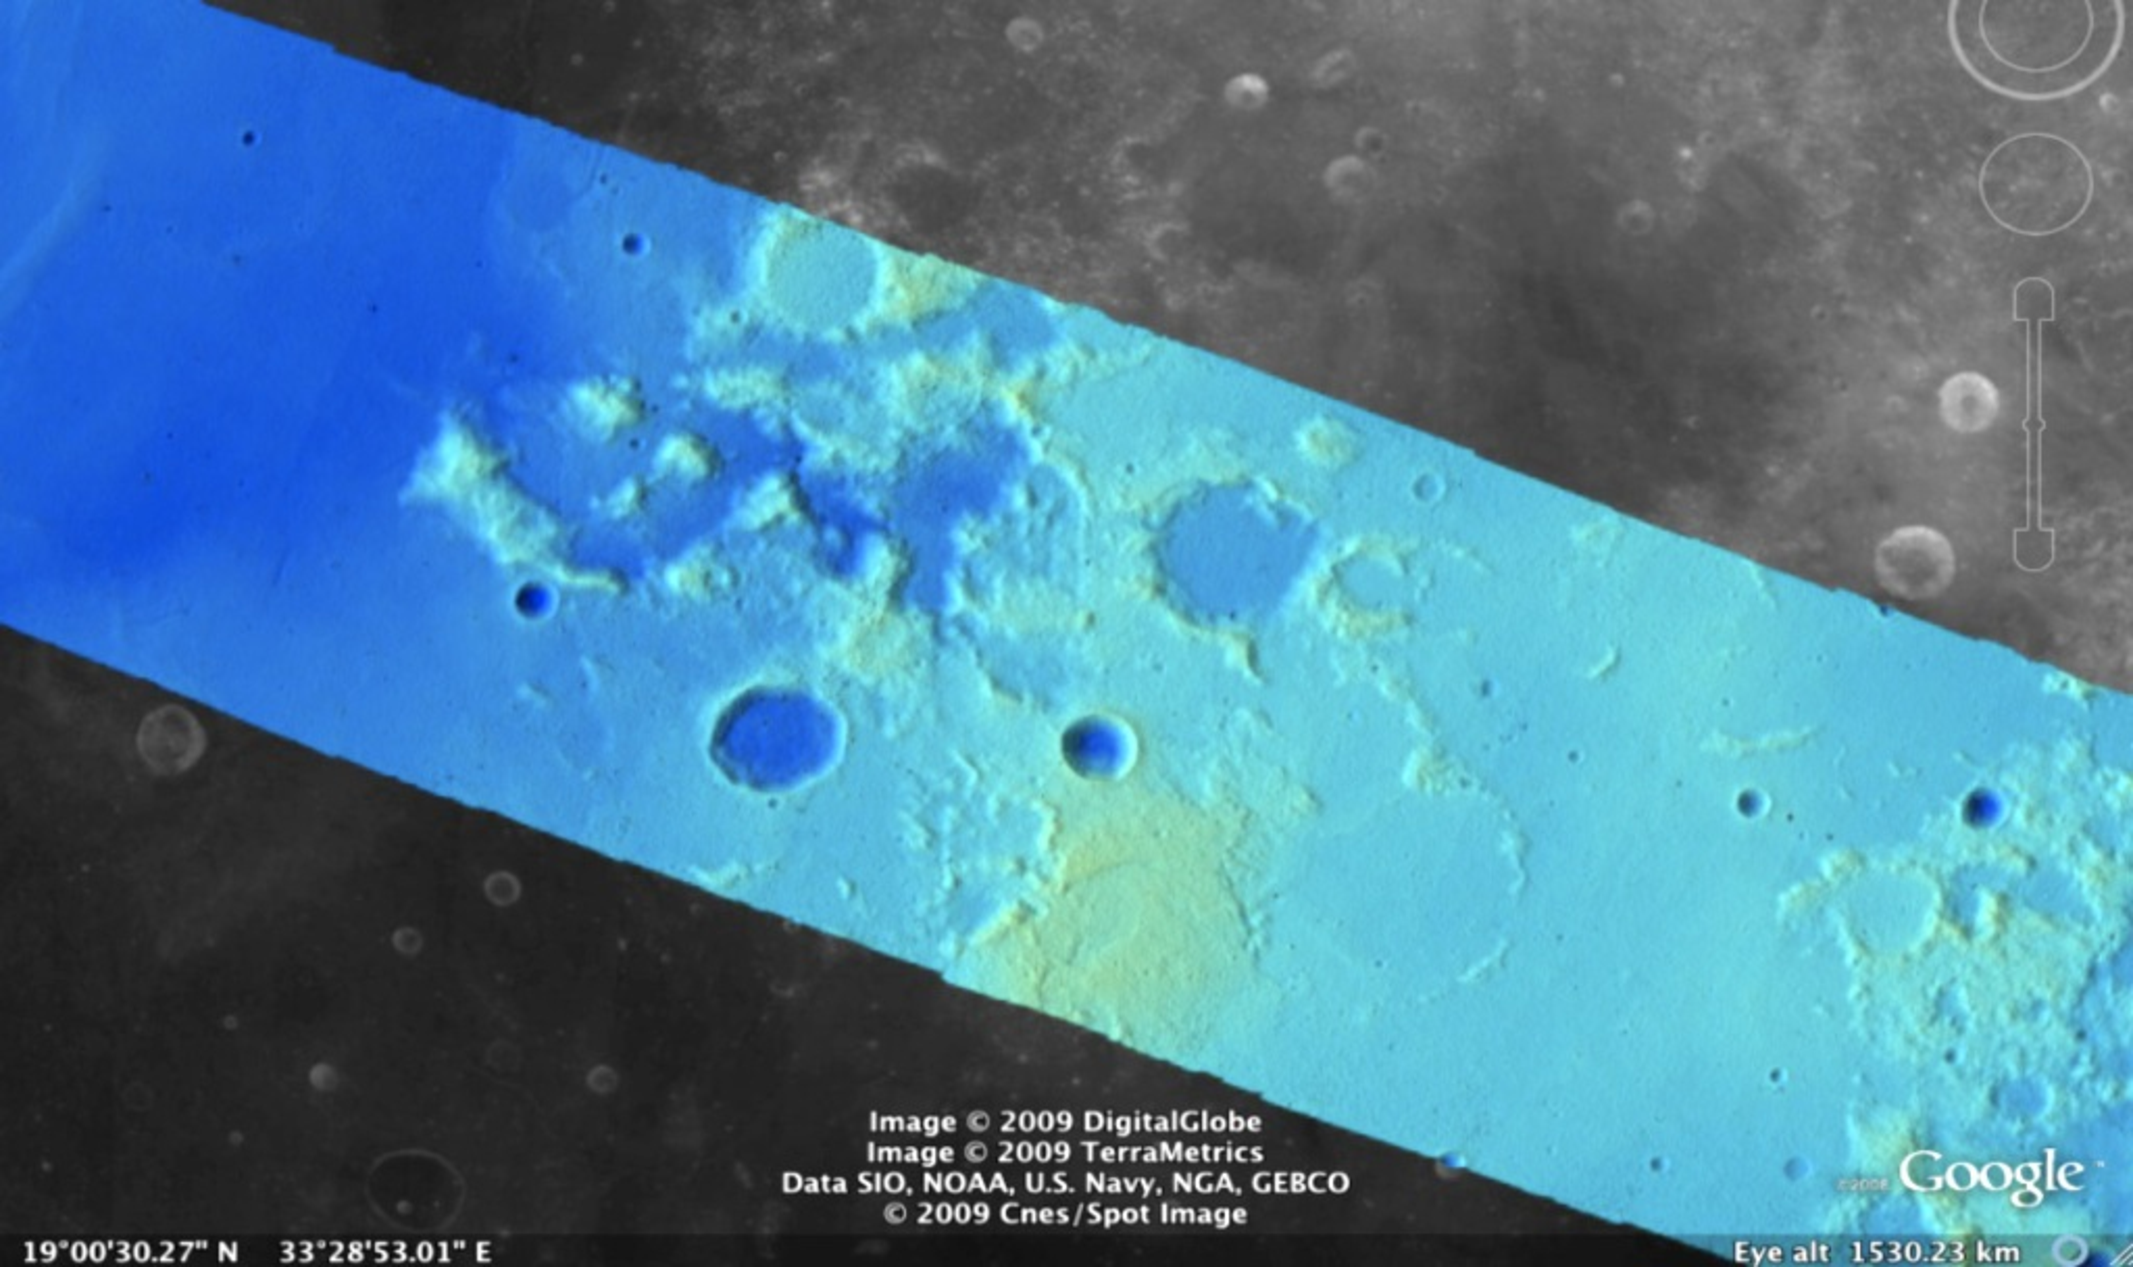
\includegraphics[width=8cm]{images/ba_adjusted}
  \caption{Bundle adjustment is illustrated here using a color-mapped,
    hill-shaded DEM mosaic from Apollo 15, Orbit 33, imagery. (a)
    Prior to bundle adjustment, large discontinuities can exist between
    overlapping DEMs made from different images. (b) After bundle
    adjustment, DEM alignment errors are minimized, and no longer visible.}
  \label{fig:bundle_adjustment}
\end{figure}

Bundle adjustment can also take advantage of \acp{GCP}, which are
3D locations of features that are known a priori (often by measuring
them by hand in another existing \ac{DEM}). \acp{GCP} can improve the internal
consistency of your \ac{DEM} or align your \ac{DEM} to an existing data
product. Finally, even though bundle adjustment calculates the
locations of the 3D objects it views, only the final properties of
the cameras are recorded for use by the Ames Stereo Pipeline. Those
properties can be loaded into the \texttt{stereo} program which
uses its own method for triangulating 3D feature locations.

When using the Stereo Pipeline, bundle adjustment is an optional step
between the capture of images and the creation of \acp{DEM}. The bundle
adjustment process described below should be completed prior to
running the \texttt{stereo} command.

Although bundle adjustment is not a required step for generating
\acp{DEM}, it is {\em highly recommended} for users who plan to
create \acp{DEM} for scientific analysis and publication.  Incorporating
bundle adjustment into the stereo work flow not only results in
\acp{DEM} that are more internally consistent, it is also the correct
way to co-register your \acp{DEM} with other existing data sets and
geodetic control networks.

At the moment however, Bundle Adjustment does not automatically work
against outside DEMs from sources such as laser altimeters. Hand
picked \acp{GCP} are the only way for \ac{ASP} to register to those
types of sources.

\subsection{A Deeper Understanding}

In bundle adjustment the position and orientation of each camera
station are determined jointly with the 3D position of a set of image
tie-points points chosen in the overlapping regions between
images. Tie points, like they sound, tie individual camera images
together. Their physical manifestation would be a rock or small crater
than can be observed across multiple images.

Tie-points can be automatically extracted using Vision Workbench's
Interest Point module, \ac{ISIS}'s \texttt{autoseed} and \texttt{pointreg},
or through a number of outside methods such as the famous
SURF\citep{surf08}. We'll be discussing the method of gathering these
measurements using \ac{ISIS}'s tool chain. Creating a collection of tie
points, {\it called a control network}, is a three step process. First, a
general geographic layout of the points must be decided upon. This is
traditionally just a grid layout that has some spacing that allows for
about a 20-30 measurements to be made per image. This decided upon grid
shows up in slightly different projected locations each image due to
their slight misalignments. The second step is have an automatic
registration algorithm try to find the same feature in all images using
the prior grid as a starting location. The third step is to manually
verify all measurements visually, checking to insure that each
measurement is looking at the same feature.

\begin{figure}[b!]
  \begin{center}
  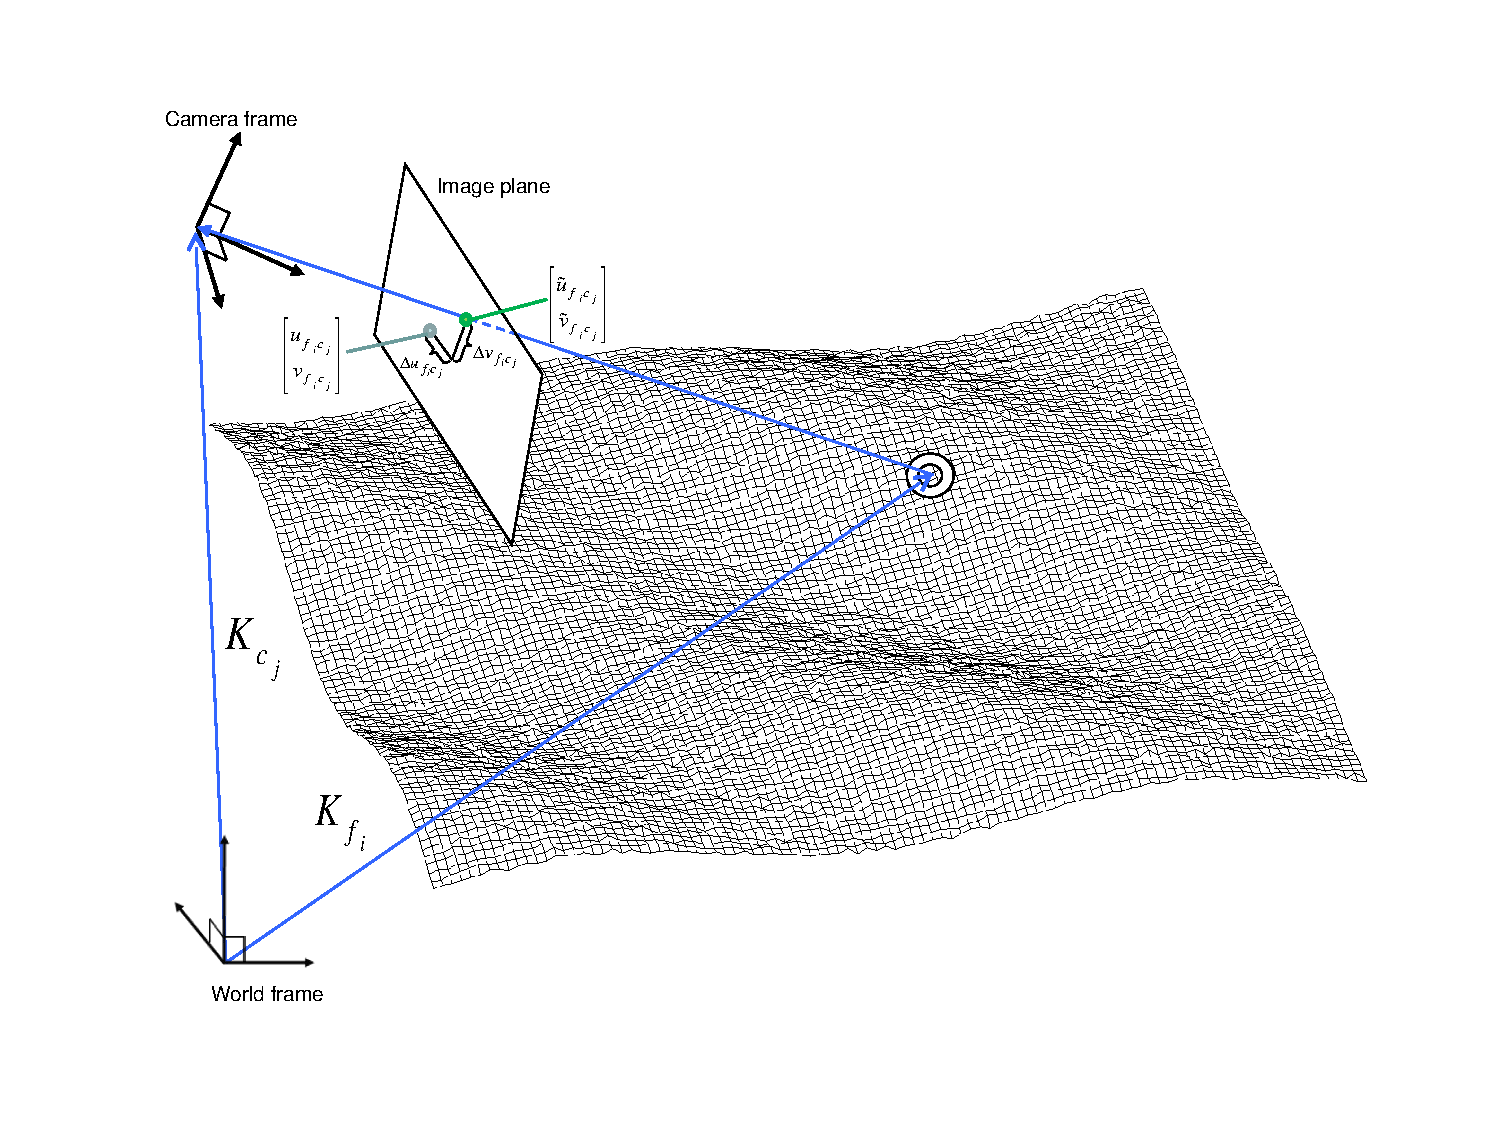
\includegraphics[trim=20mm 20mm 20mm 15mm,clip,width=6in]{images/ba_feature_observation.pdf}
  \end{center}
  \caption{ A feature observation in bundle adjustment, from \citet{moore09} }
  \label{fig:ba_feature}
\end{figure}

Bundle Adjustment in \ac{ISIS} is performed with the \texttt{jigsaw}
executable. It generally follows the method described
in~\cite{triggs00} and determines the best camera parameters that
minimize the projection error given by ${\bf \epsilon} =
\sum_k\sum_j(I_k-I(C_j, X_k))^2$ where $I_k$ are the tie points on the
image plane, $C_j$ are the camera parameters, and $X_k$ are the 3D
positions associated with features $I_k$. $I(C_j, X_k)$ is an image
formation model (i.e. forward projection) for a given camera and 3D
point. To recap, it projects the 3D point, $X_k$, into the camera with
parameters $C_j$. This produces a predicted image location for the 3D
point that is compared against the observed location, $I_k$. It then
reduces this error with the Levenberg-Marquardt algorithm (LMA). Speed
is improved by using sparse methods as described in \citet{hartley04},
\citet{konolige:sparsesparse}, and \citet{cholmod}.

Even though the arithmetic for bundle adjustment sounds clever, there
are faults with the base implementation. Imagine a case where all
cameras and 3D points were collapsed into a single point. If you
evaluate the above cost function, you'll find that the error is indeed
zero. This is not the correct solution if the images were taken
from orbit. Another example is if a translation was applied equally to
all 3D points and camera locations. This again would not affect the
cost function. This fault comes from bundle adjustment's inability to
control the scale and translation of the solution. It will correct the
geometric shape of the problem, yet it cannot guarantee that the solution
will have correct scale and translation.

\ac{ISIS} attempts to fix this problem by adding two additional cost
functions to bundle adjustment. First of which is ${\bf \epsilon} =
\sum_j(C_j^{initial}-C_j)^2$. This constrains camera parameters to
stay relatively close to their initial values. Second, a small handful
of 3D ground control points can be chosen by hand and added to the
error metric as ${\bf \epsilon} = \sum_k(X_k^{gcp}-X_k)^2$ to
constrain these points to known locations in the planetary coordinate
frame. A physical example of a ground control point could be the
location of a lander that has a well known location. GCP could also be
hand picked points against a highly regarded and prior existing map
such as the THEMIS Global Mosaic or the LRO-WAC Global Mosaic.

Like other iterative optimization methods, there are several
conditions that will cause bundle adjustment to terminate. When
updates to parameters become insignificantly small or when the error,
${\bf \epsilon}$, becomes insignificantly small, then the algorithm
has converged and the result is most likely as good as it will get.
However, the algorithm will also terminate when the number of
iterations becomes too large, in which case bundle adjustment may or
may not have finished refining the parameters of the cameras.

\section{Performing bundle adjustment with USGS's ISIS}

Ames Stereo Pipeline at one point provided its own bundle adjustment
utilities but at this point it is of our opinion that they not be used
for general use. USGS's \ac{ISIS} bundle adjustment software has
improved and gets more regular service than we could hope to provide.

This tutorial for ISIS's bundle adjustment tools is taken from
\cite{lunokhod:controlnetwork} and \cite{lunokhod:gcp}. These tools
are not a product of NASA nor the authors of Stereo Pipeline. They
were created by USGS and their documentation is available at
\cite{isis:documentation}.

\subsection{Processing Mars Orbital Camera Imagery}
\label{sec:ba_example}

What follows is an example of bundle adjustment using two \ac{MOC}
images of Hrad Vallis. We use images E02/01461 and M01/00115, the same
as used in Chapter~\ref{ch:moc_tutorial}. These images are available from
NASA's \ac{PDS} (the \ac{ISIS} \texttt{mocproc} program will operate
on either the IMQ or IMG format files, we use the \texttt{.imq} below
in the example).  For reference, the following \ac{ISIS} commands are
how to convert the \ac{MOC} images to \ac{ISIS} cubes.

\begin{verbatim}
  ISIS 3> mocproc from=e0201461.imq to=e0201461.cub mapping=no
  ISIS 3> mocproc from=m0100115.imq to=m0100115.cub mapping=no
\end{verbatim}

Note that the resulting images are not map-projected. Bundle
adjustment requires the ability to project arbitrary 3D points into
the camera frame. The process of map-projecting an image dissociates
the camera model from the image. Map-projecting can be perceived as
the generation of a new infinitely large camera sensor that may be
parallel to the surface, a conic shape, or something more
complex. That makes it extremely hard to project a random point into
the camera's original model. The math would follow the transformation
from projection into the camera frame, then projected back down to
surface that ISIS uses, then finally up into the infinitely large
sensor. \texttt{Jigsaw} does not support this and thus does not
operate on map-projected imagery.

Before we can dive into creating our tie-point measurements we must
finish prepping these images. The following commands will add a vector
layer to the cube file that describes its outline on the globe. It
will also create a data file that describes the overlapping sections
between files.

\begin{verbatim}
  ISIS 3> footprintinit from=e0201461.cub
  ISIS 3> footprintinit from=m0100115.cub
  ISIS 3> echo *cub |  xargs -n1 echo > cube.lis
  ISIS 3> findimageoverlaps from=cube.lis overlaplist=overlap.lis
\end{verbatim}

At this point, we are ready to start generating our measurements. This
is a three step process that requires defining a geographic pattern
for the layout of the points on the groups, an automatic registration
pass, and finally a manual clean up of all measurements. Creating the
ground pattern of measurements is performed with \texttt{autoseed}. It
requires a settings file that defines the spacing in meters between
measurements. For this example, write the following text into a
\textit{autoseed.def} file.

\begin{verbatim}
  Group = PolygonSeederAlgorithm
        Name = Grid
        MinimumThickness = 0.01
        MinimumArea = 1
        XSpacing = 1000
        YSpacing = 2000
  End_Group
\end{verbatim}

The minimum thickness defines the minimum ratio between the sides of
the region that can have points applied to it. A choice of 1 would
define a square and anything less defines thinner and thinner
rectangles. The minimum area argument defines the minimum square
meters that must be in an overlap region. The last two are the spacing
in meters between control points. Those values were specifically
chosen for this pair so that about 30 measurements would be produced
from \texttt{autoseed}. Having more control points just makes for more
work later on in this process. Run \texttt{autoseed} with the
following instruction.

\begin{figure}[ht]
  \centering
  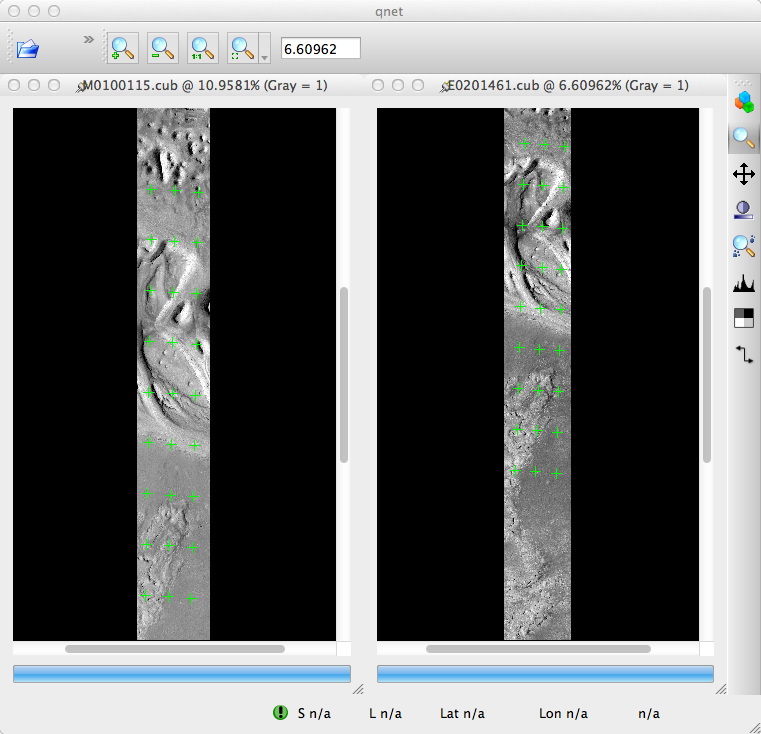
\includegraphics[width=5in]{images/qnet/Qnet_AfterAutoseed.png}
  \caption{A visualization of the features laid out by
    \texttt{autoseed} in \texttt{qnet}. Note that the marks do not
    cover the same features between images. This is due to the poor
    initial spice data for MOC imagery.}
  \label{fig:after_autoseed}
\end{figure}

\begin{verbatim}
  ISIS 3> autoseed fromlist=cube.lis overlaplist=overlap.lis    \
            onet=control.net deffile=autoseed.def networkid=moc \
            pointid=???? description=hrad_vallis
\end{verbatim}

The next step is to perform auto registration of these features
between the two images using \texttt{pointreg}. This program also
requires a settings file that describes how to do the automatic
search. Copy the text box below into a \textit{autoRegTemplate.def}
file.

\begin{verbatim}
   Object = AutoRegistration
    Group = Algorithm
      Name         = MaximumCorrelation
      Tolerance    = 0.7
    EndGroup

    Group = PatternChip
      Samples = 21
      Lines   = 21
      MinimumZScore = 1.5
      ValidPercent = 80
    EndGroup

    Group = SearchChip
      Samples = 75
      Lines   = 1000
    EndGroup
  EndObject
\end{verbatim}

The search chip defines the search range for which \texttt{pointreg}
will look for matching imagery. The pattern chip is simply the kernel
size of the matching template. The search range is specific for this
image pair. The control network result after \texttt{autoseed} had a
large vertical offset in the ball park of 500 px. The large
misalignment dictated the need for the large search in the lines
direction. Use \texttt{qnet} to get an idea for what the pixel shifts
look like in your stereo pair to help you decide on a search range. In
this example, only one measurement failed to match automatically. Here
are the arguments to use in this example of \texttt{pointreg}.

\begin{verbatim}
  ISIS 3> pointreg fromlist=cube.lis cnet=control.net             \
             onet=control_pointreg.net deffile=autoRegTemplate.def
\end{verbatim}

The third step is to manually edit the control and verify the
measurements in \texttt{qnet}. Type \texttt{qnet} in the terminal and
then open \textit{cube.lis} and lastly
\textit{control\_pointreg.net}. From the Control Network Navigator
window, click on the first point listed as \textit{0001}. That opens a
third window called the Qnet Tool. That window will allow you to play
a flip animation that shows alignment of the feature between the two
images. Correcting a measurement is performed by left clicking in the
right image, then clicking \textit{Save Measure}, and finally
finishing by clicking \textit{Save Point}.

In this tutorial, measurement \textit{0025} ended up being
incorrect. Your number may vary if you used different settings than
the above or if MOC spice data has improved since this writing. When
finished, go back to the main Qnet window. Save the final control
network as \textit{control\_qnet.net} by clicking on \textit{File},
and then \textit{Save As}.

\begin{figure}[ht]
  \centering
  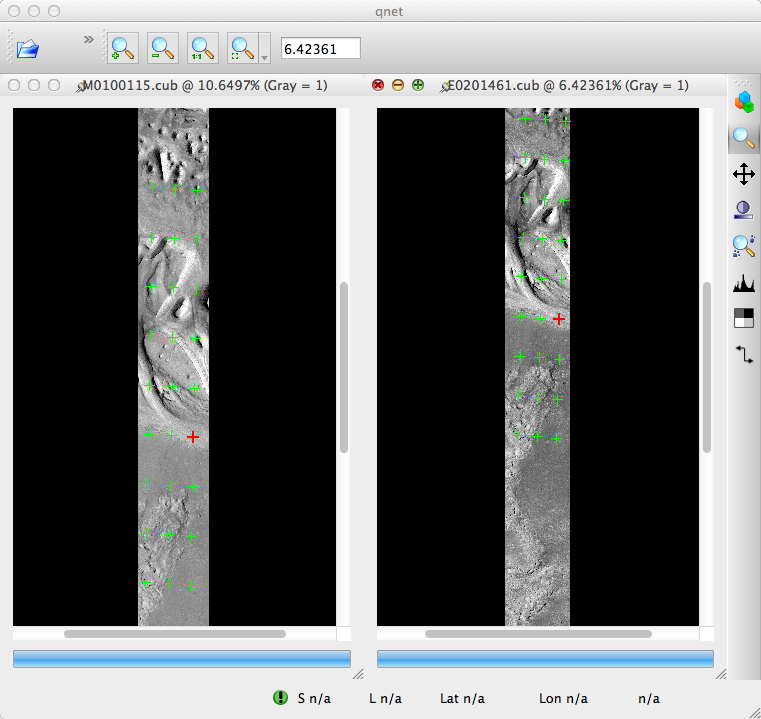
\includegraphics[width=5in]{images/qnet/Qnet_AfterQnetManual.png}
  \caption{A visualization of the features after manual editing in
    \texttt{qnet}. Note that the marks now appear in the same location
    between images.}
  \label{fig:after_manual}
\end{figure}

Once the control network is finished, it is finally time to start
bundle adjustment. Here's what the call to \texttt{jigsaw} looks like:

\begin{verbatim}
  ISIS 3> jigsaw fromlist=cube.lis update=yes twist=no radius=yes \
             cnet=control_qnet.net onet=control_ba.net
\end{verbatim}

The update option defines that we would like to update the camera
pointing, if our bundle adjustment converges. The \textit{twist=no}
says to not solve for the camera rotation about the camera bore. That
property is usually very well known as it is critical for integrating
an image with a line-scan camera. The \textit{radius=yes} means that
the radius of the 3D features can be solved for. Using no will force
the points to use height values from another source, usually LOLA or
MOLA.

The above command will spew out a bunch of diagnostic information from
every iteration of the optimization algorithm. The most important
feature to look at is the \textit{sigma0} value. It represents the mean of
pixel errors in the control network. In our run, the initial error was
1065 px and the final solution had an error of 1.1 px.

Producing a DEM using the newly created camera corrections is the same
as covered in the Tutorial on page \pageref{ch:moc_tutorial}. When using
\texttt{jigsaw}, it modifies a copy of the spice data that is stored
internally to the cube file. Thus when we want to create a DEM using
the correct camera geometry, no extra information needs to be given to
\texttt{stereo} since it is already contained in the file. In the
event a mistake has been made, \texttt{spiceinit} will overwrite the
spice data inside a cube file and provide the original uncorrected
camera pointings.

\begin{verbatim}
  ISIS 3> stereo E0201461.cub M0100115.cub bundled/bundled
\end{verbatim}

%% \subsection{Processing with Ground Control Points}

%% Ground control point files describe a single point in the world
%% that is seen by 1 or more cameras. How they are measured in the
%% first place is up to the user. We use a manual process of comparing
%% each image to a respected map-projected image and then recording
%% the latitude, longitude, and altitude of the point(s). The maps to
%% register against can be anything, but it is recommended to register
%% against a product with a high amount of cartographic stability and
%% accuracy.  For terrestrial work, we would use a \ac{USGS} product
%% that can provide imagery that is registered to LIDAR height
%% measurements.

%% Unlike match files, ground control points must specifically be given
%% to \texttt{isis\_adjust} from the command line, but in no particular
%% order. Ground control point files are written with the extension
%% \texttt{.gcp}. Below is an example of a ground control point file that
%% was created to control a series of Apollo Metric Camera images from
%% several Apollo 15 orbits.

%% \begin{verbatim}
%%     -52.8452 27.2561 1735999 300 300 500
%%     sub4-AS15-M-2086.cub     210.9   3565.0
%%     sub4-AS15-M-2087.cub     1476.9  3579.0
%%     sub4-AS15-M-2088.cub     2798.9  3586.8
%%     sub4-AS15-M-2089.cub     4133.5  3588.6
%%     sub4-AS15-M-2344.cub     906.9   3874.8
%%     sub4-AS15-M-2345.cub     2204.2  3913.9
%%     sub4-AS15-M-2482.cub     939.8   4348.0
%%     sub4-AS15-M-2483.cub     2282.0  4340.7
%%     sub4-AS15-M-2484.cub     3642.1  4330.9
%% \end{verbatim}

%% The first line of a \texttt{.gcp} file is like a header line and
%% is different from the remaining lines.  The first line defines the
%% world location of the ground control point, and the rest of the
%% lines define the image locations of the ground control points. Here
%% are what the columns mean for the first line.

%% \begin{myindentpar}{2cm}
%% \begin{description}
%%   \item[Column 1:] Longitude in degrees
%%   \item[Column 2:] Latitude in degrees
%%   \item[Column 3:] Radius in meters
%%   \item[Column 4:] Sigma (or uncertainty) in meters for Local X axis
%%   \item[Column 5:] Sigma (or uncertainty) in meters for Local Y axis
%%   \item[Column 6:] Sigma (or uncertainty) in meters for Local Z axis
%% \end{description}
%% \end{myindentpar}

%% The other lines describe where this \ac{GCP} is found in each image:

%% \begin{myindentpar}{2cm}
%% \begin{description}
%%   \item[Column 1:] Image name
%%   \item[Column 2:] Sample (X) image measurement
%%   \item[Column 3:] Line (Y) image measurement
%% \end{description}
%% \end{myindentpar}

%% Make a {\tt .gcp} file for every ground control point, then be sure
%% to feed them as an input to {\tt isis\_adjust}. Remember that you
%% can scale the sigma of all ground control points by using the {\tt
%% -\/-gcp-scalar} flag. This can save time by allowing you to make
%% adjustments without needing to edit all of the files individually.
